% !TEX program = xelatex
\documentclass{VUMIFPSkursinis}
\usepackage{algorithmicx}
\usepackage{algorithm}
\usepackage{algpseudocode}
\usepackage{amsfonts}
\usepackage{amsmath}
\usepackage{bm}
\usepackage{caption}
\usepackage{color}
\usepackage{float}
\usepackage{graphicx}
\usepackage{listings}
\usepackage{subfig}
\usepackage{array}
\usepackage{wrapfig}

\usepackage{hyperref}
\usepackage{multirow}
\usepackage{longtable}

\newcolumntype{L}[1]{>{\raggedright\let\newline\\\arraybackslash\hspace{0pt}}m{#1}}
\newcolumntype{C}[1]{>{\centering\let\newline\\\arraybackslash\hspace{0pt}}m{#1}}
\newcolumntype{R}[1]{>{\raggedleft\let\newline\\\arraybackslash\hspace{0pt}}m{#1}}

% Titulinio aprašas
\university{Vilniaus universitetas}
\faculty{Matematikos ir informatikos fakultetas}
\department{}
\papertype{Reikalavimų inžinerijos laboratorinis darbas}
\title{Reikalavimų specifikacija}
\titleineng{Requirement specification}
\status{1 kurso magistratūros studentai}
\author{Šarūnas Kazinieras Buteikis}
\secondauthor{Matas Savickis}
\thirdauthor{Rokas Ulickas}
\fourthauthor{Vytautas Krivickas}
\supervisor{dr. Audronė Lupeikienė}
\date{Vilnius – \the\year}

% Nustatymai
% \setmainfont{Palemonas} % Pakeisti teksto šriftą į Palemonas (turi būti įdiegtas sistemoje)
\bibliography{bibliografija}

\begin{document}

\maketitle

\sectionnonumnocontent{Santrauka}

Šiame dokumente pateikiama „Epidemiologinės šalies sitaucijos sekimo sistemos“
reikalavimų specifikacija. Komandą sudarė:
\begin{itemize}
	\item Šarūnas Kazinieras Buteikis (el. paštas \href{mailto:sarunas.buteikis@mif.stud.vu.lt}{sarunas.buteikis@mif.stud.vu.lt}) -- dokumento maketavimas, taisymai  {\color{red}<...>}
	\item Vytautas Krivickas (el. paštas \href{mailto:vytautas.krivickas@mif.stud.vu.lt}{vytautas.krivickas@mif.stud.vu.lt}) -- dokumento maketavimas, įžanga, {\color{red}<...>}
	\item Matas Savickis (el. paštas \href{mailto:matas.savickis@mif.stud.vu.lt}{matas.savickis@mif.stud.vu.lt}) -- dokumento maketavimas, {\color{red}<...>}
	\item Rokas Ulicas (el. paštas \href{mailto:rokas.ulickas@mif.stud.vu.lt}{rokas.ulickas@mif.stud.vu.lt}) -- {\color{red}<...>}
\end{itemize}

\newpage

\tableofcontents

\section{Įžanga}
Šiame dokumente aprašoma “Epidemiologinės šalies sitaucijos sekimo sistema”, toliau - “sistema”.
Ši sistema skirta sekti epidemiologinei padėčiai šalyje: įvertinti viruso plitimo šalyje tendencijas,
efektyviai identifikuoti naujus viruso židinius, leisti specialistams atsekti susirgusiųjų
kontaktus registruojant užsikrėtusiųjų maršrutus ir potencialiuose rizikos židiniuose
besilankančius žmones, greitai informuoti kontaktavusiuosius su užsikrėtusiu žmogumi
apie privalomą saviizoliaciją, rinkti duomenis apie asmenis karantine.

\subsection{Application domain}
Ši sistema skirta naudoti sveikatos apsaugos sistemoje: sistema turėtų palengvinti
epidemiologų darbą ir leisti sekti viruso plitimą populiacijoje, imtis efektyvesnės
profilaktikos ir tirti naudojamų priemonių efektyvumą.

\subsection{Problem domain}
Sistema siekiama išspręsti šias problemas:
\begin{itemize}
	\item Atskirų sveikatos įstaigų renkami susirgimų duomenys nėra apdorojami centralizuotai
	      arba tai daroma ne sistemingai, todėl epidemiologams sunku identifikuoti tikrąsias viruso
	      plitimo šalyje tendencijas, greitai identifikuoti potencialius židinius.
	\item Dėl žmogiškųjų resursų trūkumo dažnai tampa neįmanoma įspėti visų kontaktavusiųjų
	      su užsikrėtusiuoju asmenų - automatizavus šį procesą būtų galima įgyvendinti efektyvesnę
	      profilaktiką, užkardyti nevaldomą epidemijos plitimą.
	\item Šiuo metu nėra centralizuotos sistemos, leidžiančios registruoti potencialiuose
	      rizikos židiniuose (įvairuose renginiuose, masinio susibūrimo vietose) besilankančius
	      asmenis, dabar egzistuojančios pavienės iniciatyvos neleidžia automatiškai atsekti reikšmingo kiekio susirgusiojo kontaktų - tenka pasikliauti pastarojo pateikta informacija.
	\item Nacionalinio sveikatos centro darbuotojai neturi galimybės automatiškai įspėti
	      atvykusiųjų iš pavojingų šalių asmenų apie privalomą saviizoliaciją: atlikus reikiamas
	      integracijas su {\color{red}muitinės (?)} sistemomis ši sistema leistų automatizuoti ir šį procesą.
	\item Šiuo metu nėra galimybės automatizuoti saviizoliacijos reikalavimų laikymosi sekimo,
	      tad naujoji sistema leistų bent iš dalies automatizuoti šį procesą: reikalauti asmenis
	      saviizoliacijoje pateikti savo dabartinę vietą naudojantis išmaniajame telefone esančia
	      GPS sistema ar atsiųsti saviizoliaciją patvirtinančią nuotrauką.
\end{itemize}

\subsection{Naudotojai}
Šios sistemos naudotojų bazę sudaro trijų kategorijų naudotojai:
\begin{itemize}
	\item Epidemiologai - tai savo srities ekspertai, turintys aukštąjį išsilavinimą.
	      Naudotis sistema jiems pakaks mokykloje dėstomo informatikos kurso.
	\item LR esantys asmenys, dalyvaujantys riziką turinčiuose renginiuose, esantys saviizoliacijoje,
	      atvykę iš pavojingų šalių ar turėję sąlytį su sergančiaisiais - jiems taip pat pakaks
	      mokykloje dėstomo informatikos kurso.
	\item Duomenų analitikai - tam, jog galėtų efektyviai panaudoti sistemoje
	      esančius duomenis jiems reikalingas bakalauro ar aukštesnis iššsilavinimas
	      duomenų mokslo ar informatikos srityse.
\end{itemize}

\newpage

\section{Reikalavimų artefaktai}

\begin{table}[h!]
	\begin{tabular}{|p{4cm}|p{4cm}|p{4cm}|p{4cm}|}
		\hline
		                          & Kodėl? (motyvacija) & \multicolumn{1}{c|}{Kaip? (veiklos)} & Ką? (apdorojami objektai) \\ \hline
		\begin{tabular}[c]{@{}l@{}}Veikslo reikalavimai \\ (verslo inžinieriaus \\ požiūris)\end{tabular} &                     &
			1.Galimybė valdyti duomenis apie žmones susirgusius virusu.
			2.Galimybė valdyti duomenis apie naujus ligos atvejus.
			3.Galimybė registruoti užsikrėtusių žmonių maršrutus.
			4.Galimybė perduoti statistiką suinteresuotoms asmenims.
			5.Galimybė valdyti pavojingų šalių sąrašą.
			6.Galimybė valdyti informaciją apie saviizoliacijos pažeidimus.
			7.Galimybė valdyti duomenis apie iš pavojingų šalių atvykstančius asmenis.
			8.Galimybė valdyti duomenis apie masinius renginius.
			9.Galimybė valdyti duomenis apie viešojo maitinimosi įstaigas.
			10.Galimybė valdyti duomenis apie asmens rizikos faktorius.
			11.Galimybė valdyti informaciją apie asmens saviizoliacijos patvirtinimą.
			12.Galimybė valdyti asmenų sveiaktos informaciją


		                          &                                                                                        \\ \hline
	\end{tabular}
\end{table}

\begin{table}[h!]
	\begin{tabular}{|p{4cm}|p{4cm}|p{4cm}|p{4cm}|}\hline
		                          & Kodėl? (motyvacija) & \multicolumn{1}{c|}{Kaip? (veiklos)} & Ką? (apdorojami objektai) \\ \hline
		\begin{tabular}[c]{@{}l@{}}Vartotojo reikalavimai \\ (dalykinės srities \\ specialisto požiūris)\end{tabular} &  
			Epidemiloginės situacijos sekimo sistemą reikia kurti, kad būtų galima sekti ir valydti duomenis apie 
			virusu susirgusius asmenis. Sistema padėtų centralizuoti epidemijos sekimą ir įgalintų greitą komunikaciją 
			tarp suinteresuotų asmenų, pateiktų informaciją sergantiems asmenims ir taip padėtų kovoje su virusu 
			bei įgalintų efetyvesnį viruso plitimo valdymą.             &     

			Informacija tarp suinteresuotų šalių bus apsikeičiama kompiuterizuotu, automatizuotu būdu.
			Duomenys apsikeičiami arba numatytais laiko momentais arba suinteresuotai pusei paprašius įvykdyti tranzakcija.
			Komunikacija tarp suinteresuotu šalių vyksta serverių duomenų apsikeitimo vykmenyje.
			Privatiems asmenims informacija yra perduodama trumposiomis žinutėmis, elektroniniu paštu arba asmeniniu skambučiu.
			
			                                 & 

			Sistemoje kaupsime epidemiologinius duomenis susijusius apie asmenis: kur žmogus lankėsi, jo sveikatos istorija, asmeniai duomenys, žmogaus esamą buvimo vietą , viruso testo rezultatus.
			Sistemoje kaupsime epidemiologinius duomenis apie renginius ir viešasias maitinimo įskaitas, kada kokia žmonės ten lankės, kas dalyvavo renginyje ar maitinimo istaigoje prieš susirgdamas.
			Sistemoje kaupsime epidemiologinius duomenis apie pavojingu šalių sąrašus ir žmones atvykstančius iš šių šalių, kur jie lankėsi, kiek laiko izoliavosi.
			Visi duomenys bus valdomi pagal BDAR įstatymą.
			Visus duomenis matys tik valstybinių organizacijų atsovai turintys priviliaciją matyti šiuos duomenis.                       \\ \hline
	\end{tabular}
\end{table}

\begin{table}[h!]
	\begin{tabular}{|p{4cm}|p{4cm}|p{4cm}|p{4cm}|}\hline
		                           & Kas? (funkciniai vienetai) & \multicolumn{1}{c|}{Kur? (vieta)} & Kada? (laikas) \\ \hline
		\begin{tabular}[c]{@{}l@{}}Vartotojo reikalavimai \\ (dalykinės srities \\ specialisto požiūris)\end{tabular} &  
			Sistema gali naudotis tik vartotojai turintys tinkama privilegiju lygi.
			Vartotojui neturi buti pateikta daugiau duomenu ir funkcionalumu negu nurodo jo privilegijos lygis sistemoje.
			Projektuojant sistemos prieinamuma reikia laikytis prielaidos, kad sistemos vartotojai turės bazinį informacinių technologijų raštingumo lygį.
			Po sistemos sukūrimo vartotojai bus apmokomi varottis sistema, tačiau tikimasi, kad varotojai jau bus naudojasi kitomis, panašiomis sistemomis.                          &   

			Programine sistema pasiekti galima tik nurodytoja darbo vietoje arba prisijungus į virtualų privatų tinklą(VPA) užtikrinant darbo iš namų galimybę.                              &     
			Sistema turi užtikrinti, kad jos prieeinamumas nebūtų mažesnis negu nurodyti laiko apribojimų.           \\ \hline
	\end{tabular}
\end{table}

\begin{table}[h!]
	\begin{tabular}{|p{4cm}|p{4cm}|p{4cm}|p{4cm}|}\hline
		                          & Kodėl? (motyvacija) & \multicolumn{1}{c|}{Kaip? (veiklos)} & Ką? (apdorojami objektai) \\ \hline
		\begin{tabular}[c]{@{}l@{}}IS reikalavimai \\ (IS inžinieriaus \\ požiūris)\end{tabular} &                     &                                      &                           \\ \hline
	\end{tabular}
\end{table}

\begin{table}[h!]
	\begin{tabular}{|p{4cm}|p{4cm}|p{4cm}|p{4cm}|}\hline
		                           & Kas? (funkciniai vienetai) & \multicolumn{1}{c|}{Kur? (vieta)} & Kada? (laikas) \\ \hline
		\begin{tabular}[c]{@{}l@{}}IS reikalavimai \\ (IS inžinieriaus \\ požiūris)\end{tabular} &                            &                                   &                \\ \hline
	\end{tabular}
\end{table}

\begin{table}[h!]
	\begin{tabular}{|p{4cm}|p{4cm}|p{4cm}|p{4cm}|}\hline
		                           & Kodėl? (vizija ir suvaržymai) & Kaip? (sistemos panaudojimo atvėjai ir kokybė) & Ką(duomenys ir jų sauga) \\ \hline
		\begin{tabular}[c]{@{}l@{}}Programos reikalavimai \\ (Kiekvienai sistemai)\end{tabular} & 
			Sistema bus kuriama debesijos komiuterijos pagalba pagerinti ateities išlaikymo kaštus. 
			Sistema laikysis organizacijos politinių reikalavimų ir ribojimų.
			Sistema laikysis Lietuvos ir Europos teisinių apribojimų.
			Sistemai svarbiau patikimumas, kad visi paciantai būtų užregistruoti negu našumas, vartotojas gali palaukti. & 
			
			                                  &                \\ \hline
	\end{tabular}
\end{table}

\begin{table}[h!]
	\begin{tabular}{|p{4cm}|p{4cm}|p{4cm}|p{4cm}|}\hline
		                           & Kas? (vartotojo sąsajos, prieinamumo ir ergonomikos reikalavimai) &Kur? (sistemos platformos reikalavimai) & Kada? (laiko suvaržymai aplikacijos panaudojimo atvejuose) \\ \hline
		\begin{tabular}[c]{@{}l@{}}Programos reikalavimai \\ (Kiekvienai sistemai) \end{tabular} &                            &                                   &                \\ \hline
	\end{tabular}
\end{table}



\section{Verslo reikalavimai}

\subsection{Kodėl?}

\begin{figure}[H]
    \centering
    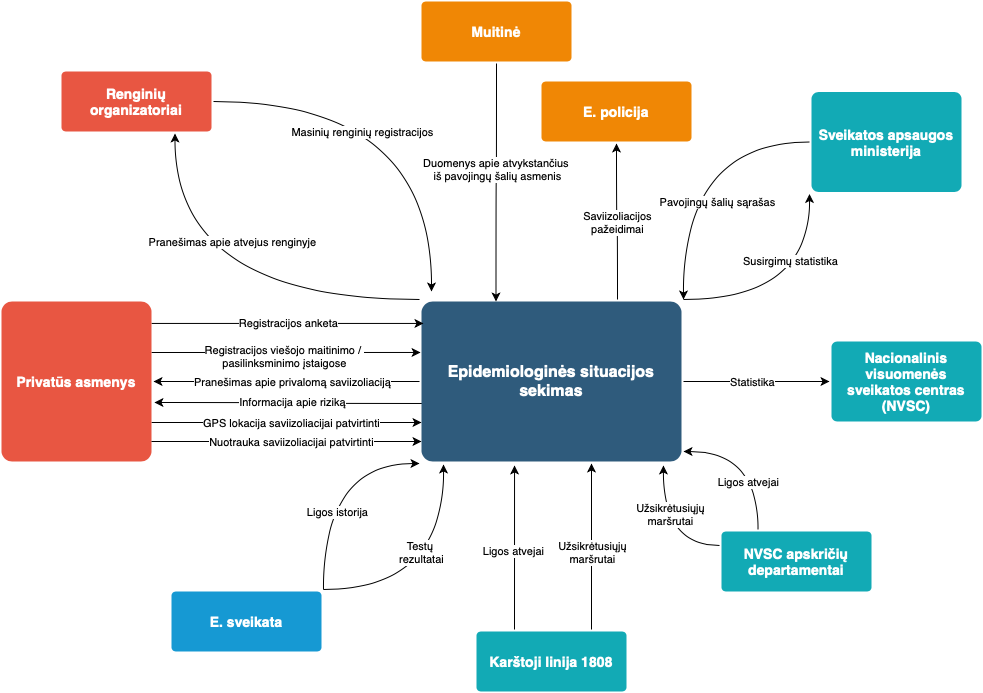
\includegraphics[scale=0.5]{img/context_diagram.png}
    \caption{Konteksto diagrama}
    \label{img:context_diagram}
\end{figure}

\subsubsection{Išorinė verslo analizė}

\begin{figure}[H]
    \centering
    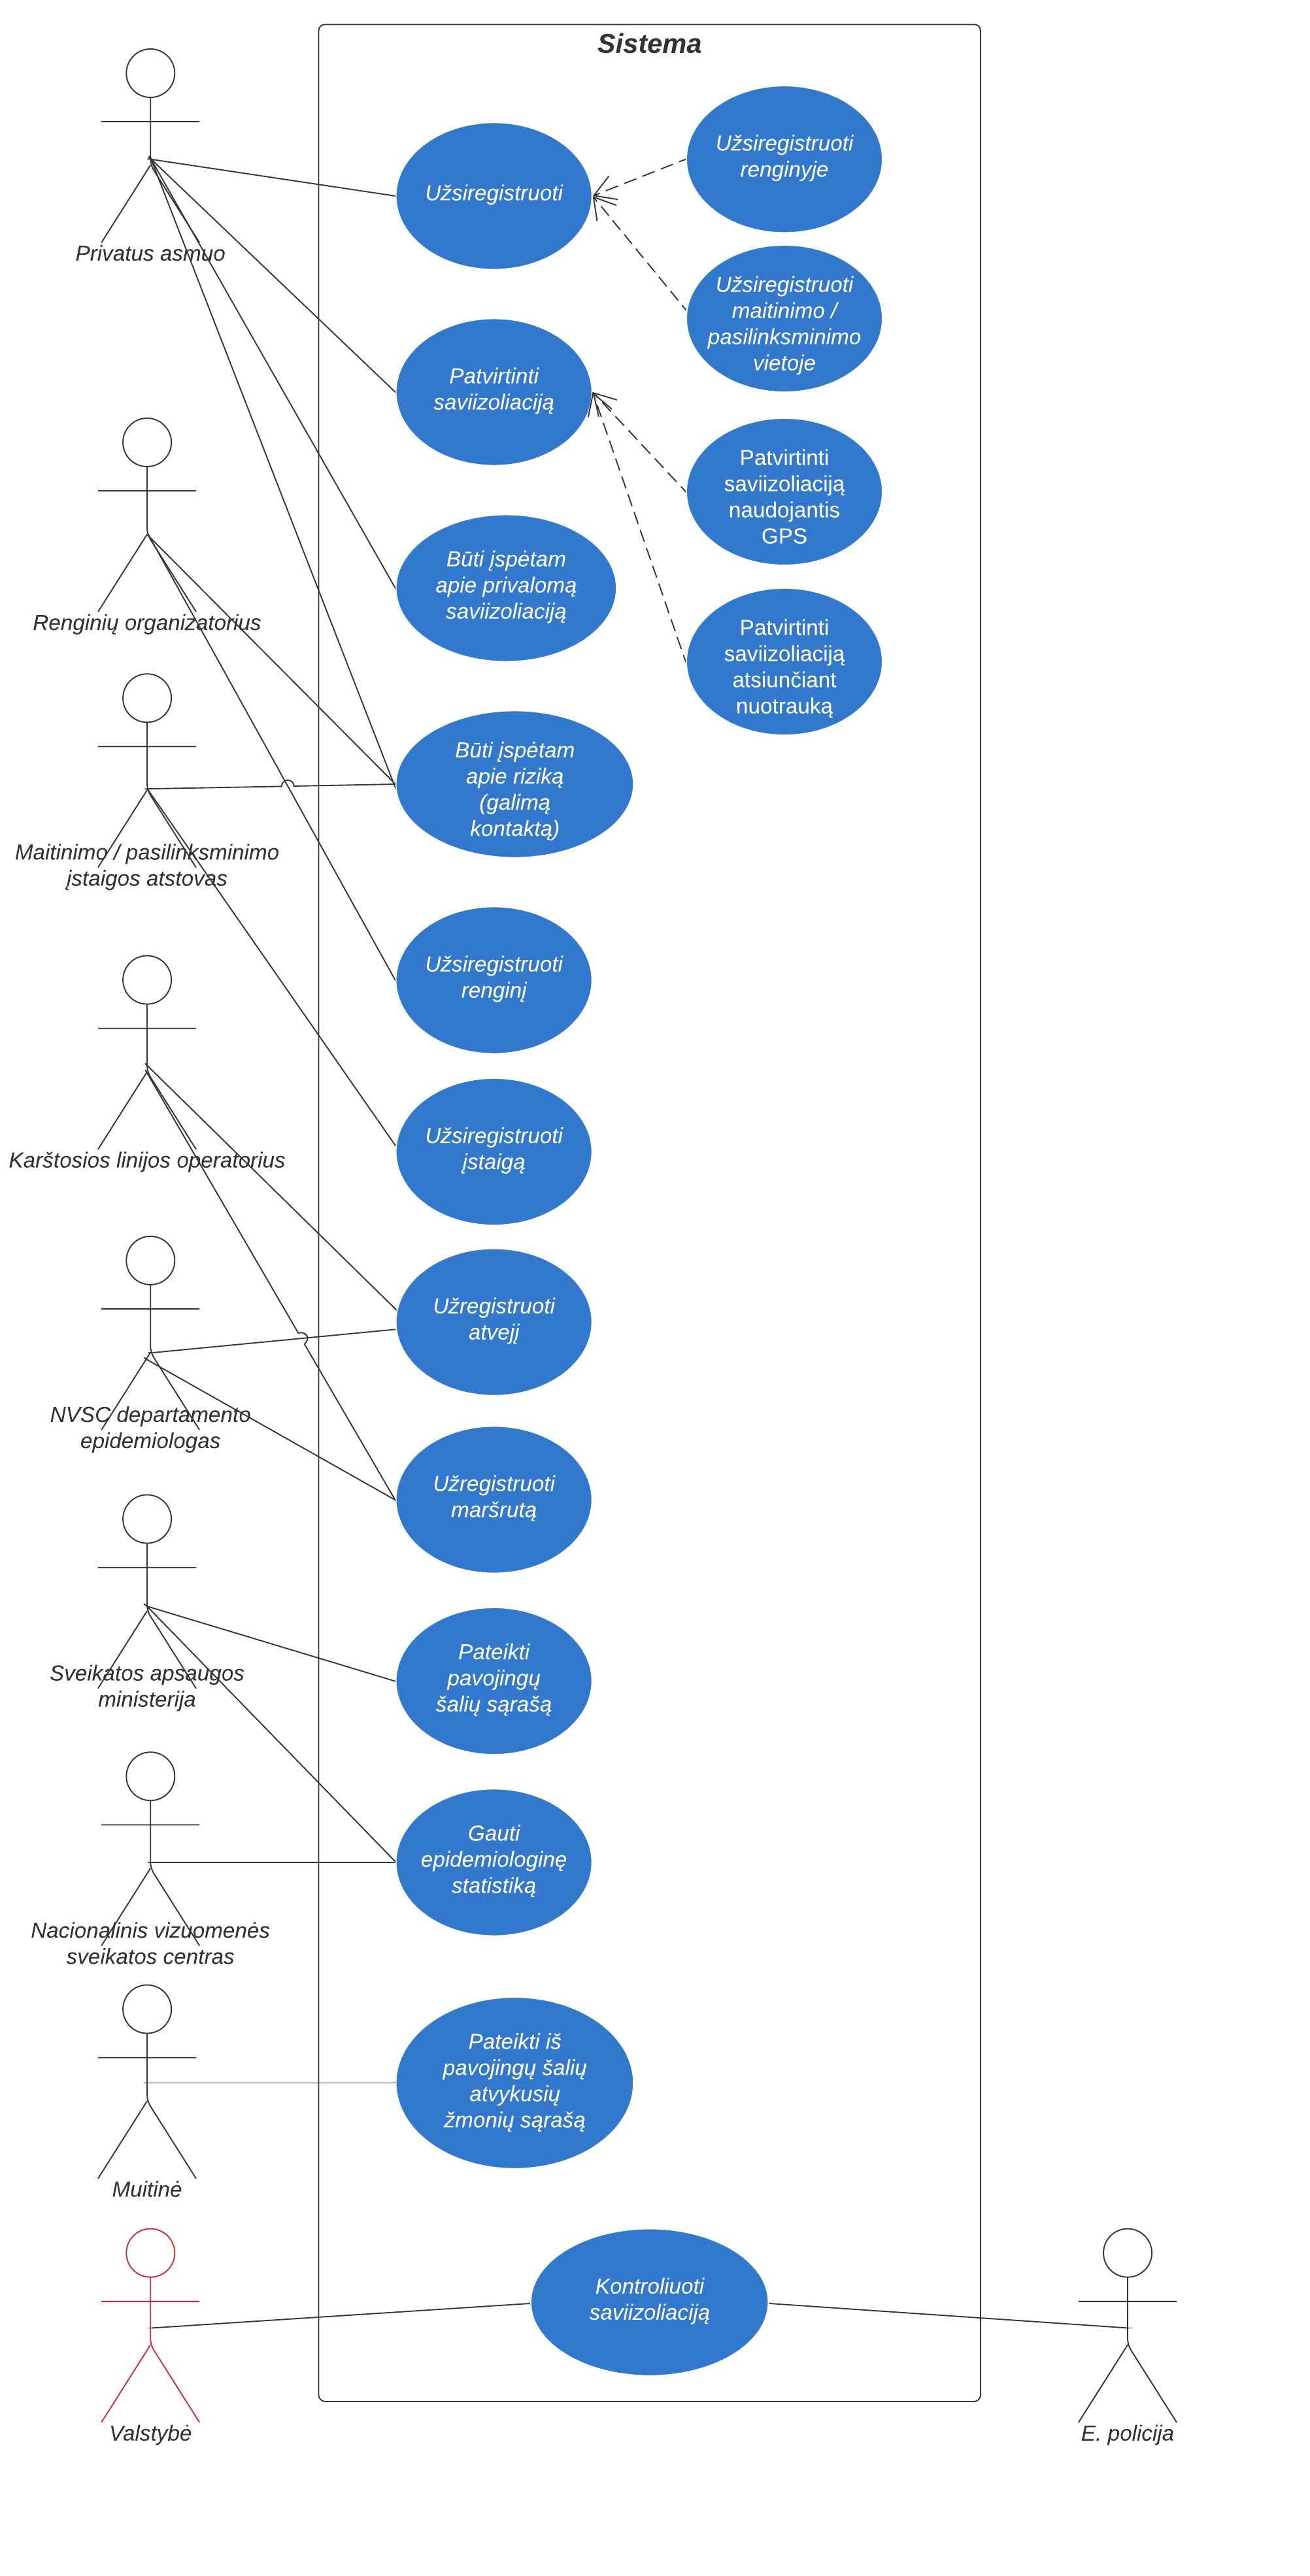
\includegraphics[scale=0.6]{img/use_case_diagram.png}
    \caption{Konteksto diagrama}
    \label{img:use_case_diagram}
\end{figure}

\subsubsection{Įvestys}

\begin{table}[]
	\centering
	\resizebox{\textwidth}{!}{%
		\begin{tabular}{|l|l|l|l|l|}
			\hline
			\textbf{Nr.}        & \textbf{Įvestis}                                            & \multicolumn{1}{c|}{\textbf{Įvertinimo parametrai}} & \multicolumn{1}{c|}{\textbf{Kiekybiniai matai}} & \multicolumn{1}{c|}{\textbf{Kokybiniai matai}} \\ \hline
			\multirow{2}{*}{I1} & \multirow{2}{*}{Registracijos didesnės rizikos renginiuose} & Kiekis                                              &                                                 &                                                \\ \cline{3-5}
			                    &                                                             & Korektiškumas                                       &                                                 &                                                \\ \hline
			I2                  & Registracijos viešojo maitinbimo įstaigose                  &                                                     &                                                 &                                                \\ \hline
			I3                  & Informacija apie keliones iš rizikos šalių                  &                                                     &                                                 &                                                \\ \hline
			I4                  & Pavojingų šalių sąrašas                                     &                                                     &                                                 &                                                \\ \hline
			I5                  & Asmenų ligos istorijos                                      &                                                     &                                                 &                                                \\ \hline
			I6                  & Testų rezultatai                                            &                                                     &                                                 &                                                \\ \hline
			I7                  & Saviizoliaciją patvirtinantys vietos nustatymo duomenys     &                                                     &                                                 &                                                \\ \hline
			I8                  & Saviizoliaciją patvirtinanti nuotrauką                      &                                                     &                                                 &                                                \\ \hline
			I9                  & Atvykusių iš pavojingų šalių žmonių sąrašas                 &                                                     &                                                 &                                                \\ \hline
			I10                 & Masinių renginių registracijos                              &                                                     &                                                 &                                                \\ \hline
			I11                 & Užsikrėtusiųjų maršrutai                                    &                                                     &                                                 &                                                \\ \hline
			I12                 & Pranešimai apie įtariamus atvejus                           &                                                     &                                                 &                                                \\ \hline
		\end{tabular}%
	}
\end{table}

\subsubsection{Išvestys}
\begin{table}[]
	\centering
	\resizebox{\textwidth}{!}{%
		\begin{tabular}{|l|l|l|l|l|}
			\hline
			\textbf{Nr} & \textbf{Išvestis}                          & Įvertinimo parametrai & Kiekybiniai matai & Kokybiniai matai \\ \hline
			\textbf{O1} & Statistika (?)                             &                       &                   &                  \\ \hline
			\textbf{O2} & Pranešimas apie priverstinę saviizoliaciją &                       &                   &                  \\ \hline
			\textbf{O3} & Pranešimas apie saviizoliacijos pažeidimą  &                       &                   &                  \\ \hline
			\textbf{O4} & Pranešimas apie riziką                     &                       &                   &                  \\ \hline
			\textbf{O5} & Pranešimas renginių org. apie atvejus      &                       &                   &                  \\ \hline
			\textbf{O6} &                                            &                       &                   &                  \\ \hline
			\textbf{O7} &                                            &                       &                   &                  \\ \hline
			\textbf{O8} &                                            &                       &                   &                  \\ \hline
			\textbf{O9} &                                            &                       &                   &                  \\ \hline
		\end{tabular}%
	}
\end{table}

\subsubsection{Reguliacija}
Sistemoje renkamų bei saugomų duomenų tvarkymą reglamentuoja Lietuvos Respublikos asmens duomenų teisinės apsaugos įstatymas,
Bendrasis duomenų apsaugos reglamentas. Saviizoliacijos tvarką bei organizatorių prievolę registruoti renginių dalyvius nustato
LR vyriausybės nutarimas dėl valstybės lygio ekstremalios situacijos paskelbimo. Atsakomybę už saviizoliacijos pažeidimus
apibrėžia baudžiamasis kodeksas.

\subsubsection{Įvaizdis}
Apibendrinant galima išskirti dvi grupes, vertinančias sistemos įvaizdį: specialistus, besinaudosiančius sistema
bei visuomenę. Abi grupės sistemos įvaizdį vertins visų pirma patikimumo aspektu: ar sistema veikia be trikdžių,
nepažeidžiamas doumenų saugumas. Specialistai taip pat įvertins sistemos efektyvumą -- kaip patogu atlikti reikiamas
užduotis bei greitį -- kaip greitai sistema veikia. Neigiamą sistemos įvaizdį visuomenėje galėtų lemti jautrių duomenų,
renkamų sistemoje, kiekis bei automatinė saviizoliacijos pažeidimų fiksavimo funkcija.

\begin{table}[]
	\centering
	\resizebox{\textwidth}{!}{%
		\begin{tabular}{|l|l|l|l|l|}
			\hline
			\textbf{Nr}                   & \textbf{Grupė}                 & Įvertinimo parametrai & Kiekybiniai matai               & Kokybiniai matai                                                                                      \\ \hline
			\textbf{IM1}                  & Visuomenė                      & Patikimumas           &                                 & Pranešimai žiniasklaidoje ar soc. tinkluose apie prastą (klaidingą, lėtą, nepatogų) sistemos veikimą. \\ \hline
			\multirow{2}{*}{\textbf{IM2}} & \multirow{2}{*}{Profesionalai} & Patikimumas           & Sistemos pasiekiamumas (uptime) & Trikdžiai ar klaidos naudojantis sistema.                                                             \\ \cline{3-5}
			                              &                                & Patogumas             & Užduočių atlikimo greitis       & Naudotojo patirtis                                                                                    \\ \hline
		\end{tabular}%
	}
\end{table}

\subsubsection{Vidinė verslo analizė}

\subsubsection{Vizija}
Tapti pagrindiniu viruso plitimo visuomenėje valdymo įrankiu specialistams.

\subsubsection{Misija}
Su viruso plitimu susijusių duomenų agregavimas, leidžiantis sekti jo plitimą, pateikti rekomendacijas,
įspėti visus rizikoje atsidūrusius asmenis, bei kontroliuoti saviizoliacijos laikymąsį.

\subsubsection{SWOT analizė}

\begin{figure}[H]
    \centering
    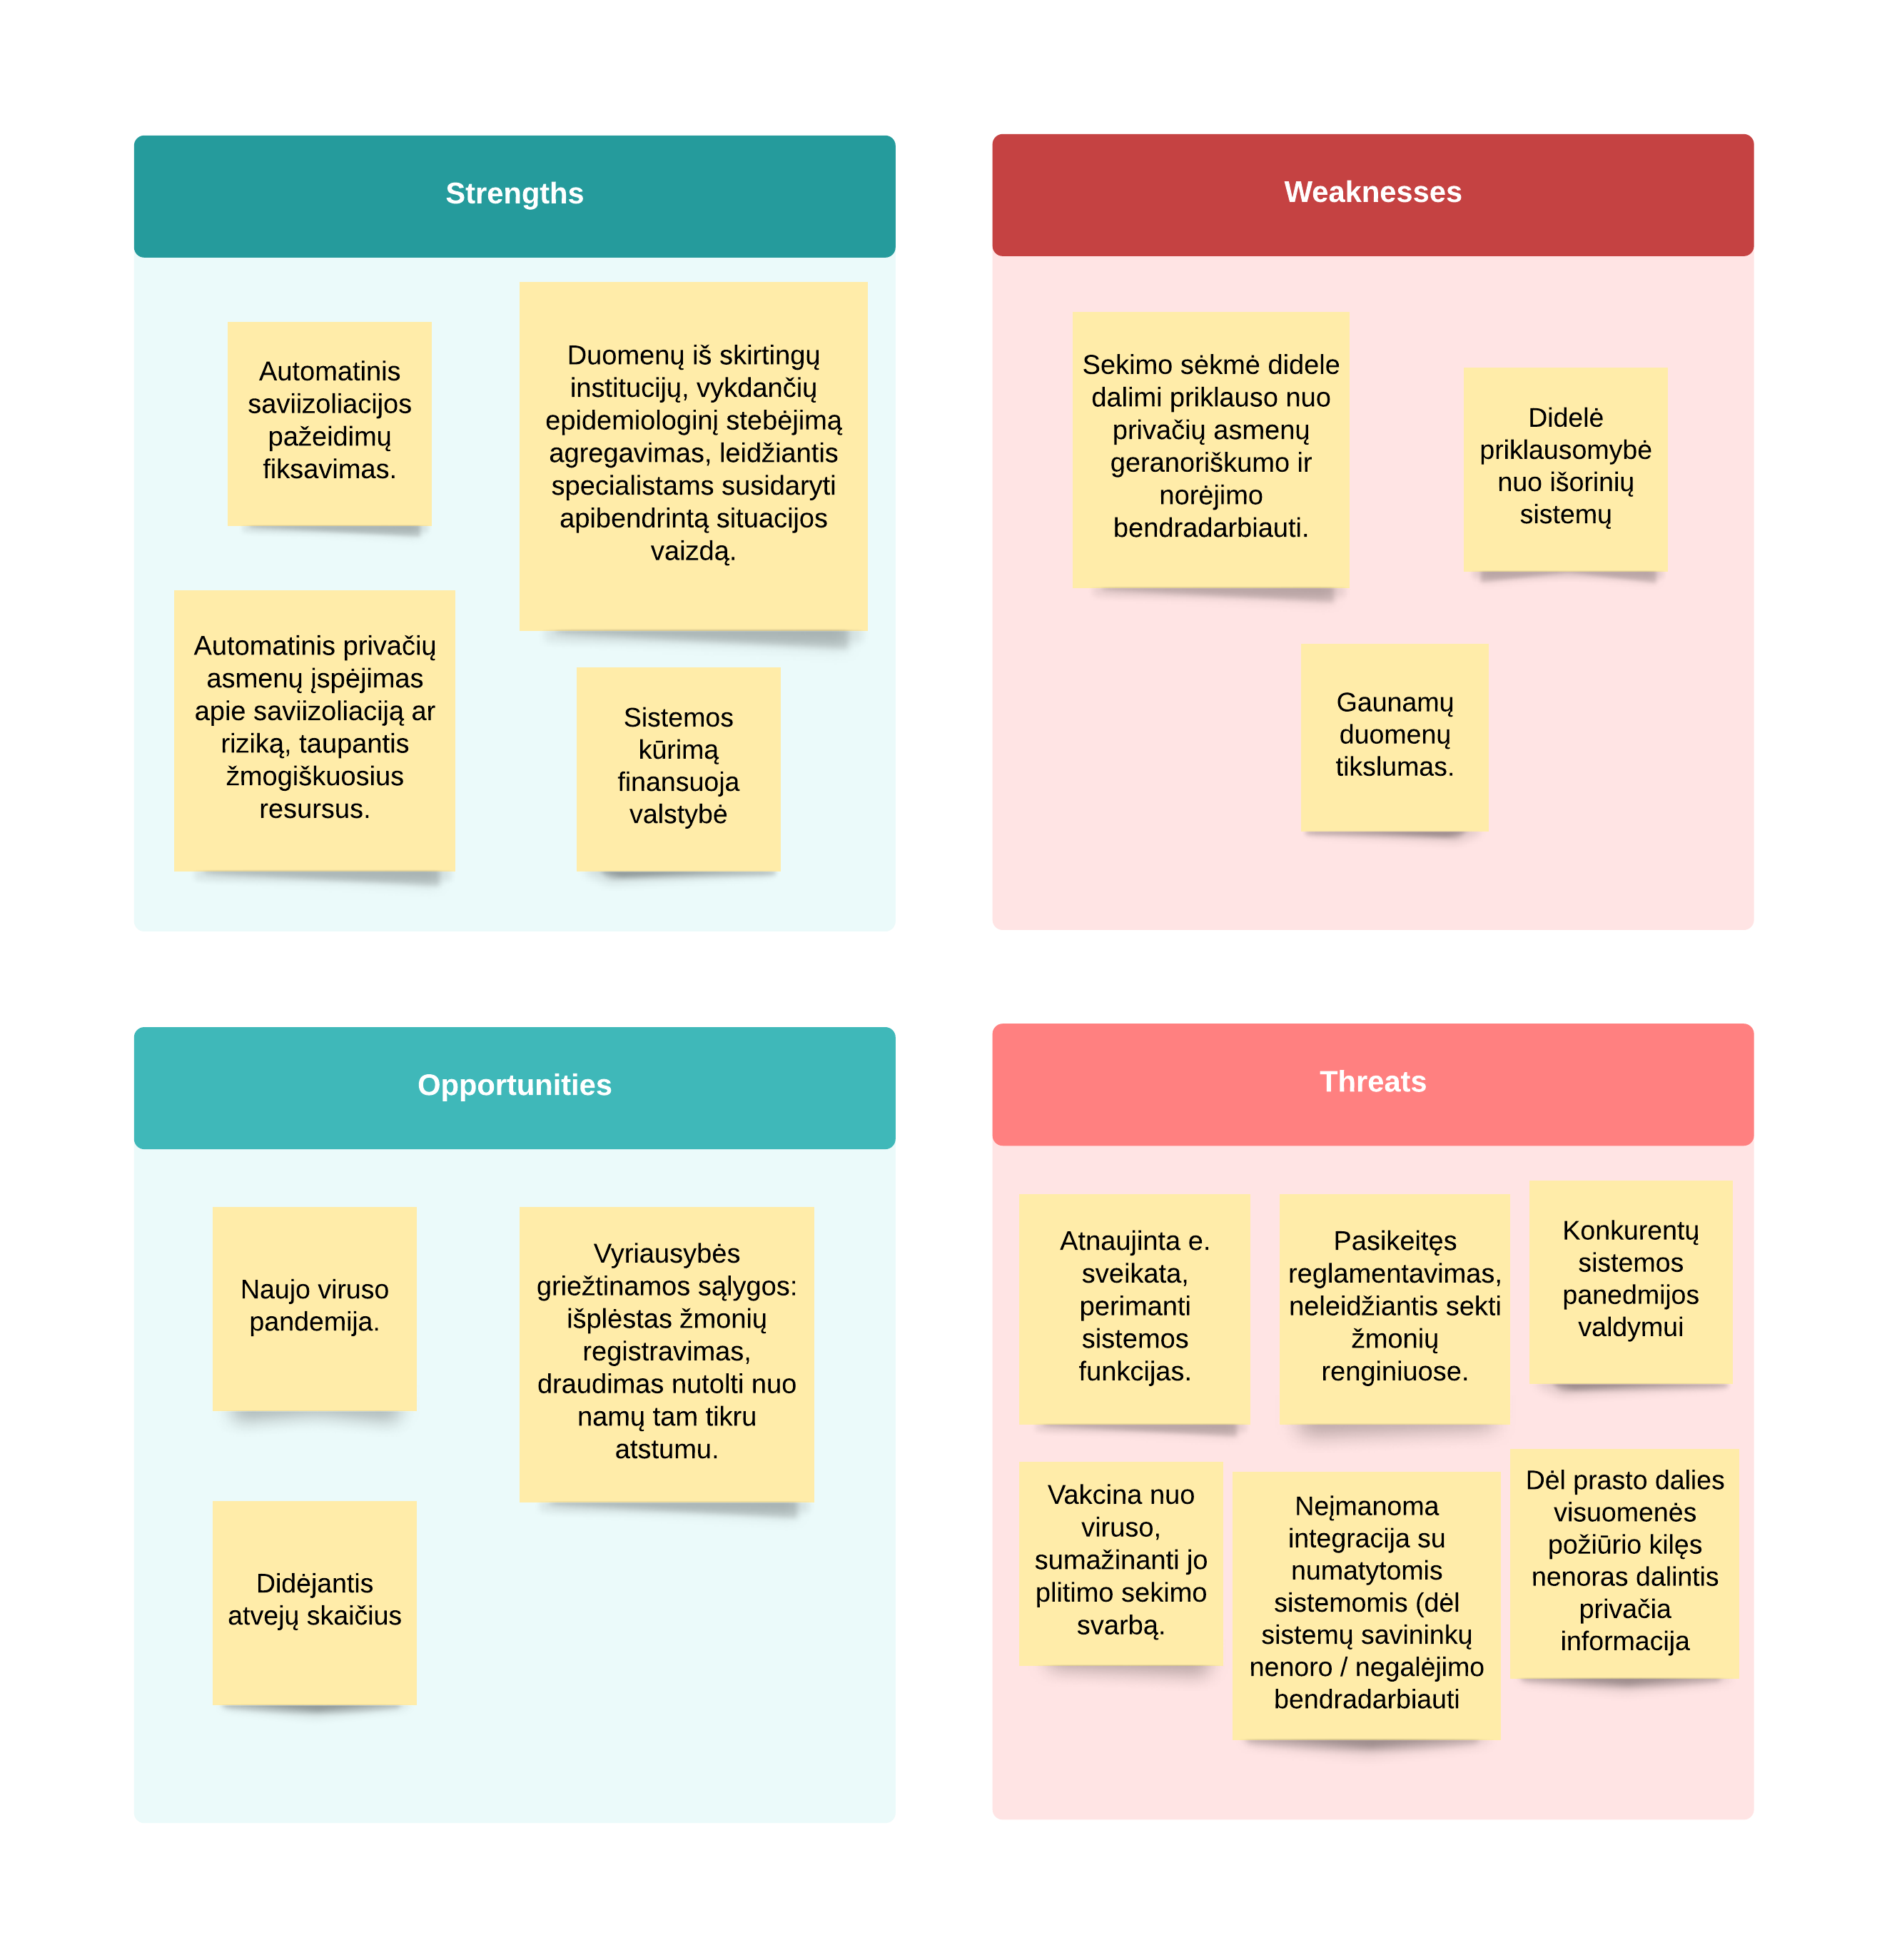
\includegraphics[scale=0.7]{img/SWOT.png}
    \caption{SWOT diagrama}
    \label{img:swot_diagram}
\end{figure}

\subsubsection{Siūloma verslo strategija}

\subsubsection{Tikslų medis}

\begin{enumerate}
	\item Pagerinti komunikaciją tarp  
	\item Tapti pagrindiniu duomenų apie viruso plitimą visuomenėje šaltiniu
		\begin{enumerate}
			\item Sukurti centralizuotą duomenų apie susirgimus registrą
			\item Sukurti centralizuotą duomenų apie maitinimo / pasilinksminimo įstaigų ir renginių lankytojus registrą
		\end{enumerate}
	\item Atlikti viruso plitimo prevenciją
	\begin{enumerate}
		\item Įspėti privačius asmenis apie riziką
		\item Įspėti organizatorius apie atvejus renginiuose / įstaigose
	\end{enumerate}
	\item Užtikrinti saviizoliacijos laikymąsi.
	\begin{enumerate}
		\item Pranešti apie privalomą saviizoliaciją.
		\begin{enumerate}
			\item Gauti pavojingų šalių sąrašą.
			\item Gauti atvykstančių žmonių sąrašą.
		\end{enumerate} 
		\item Tikrinti saviizoliacijos laikymąsi.
		\begin{enumerate}
			\item Registruoti GPS duomenis.
			\item Tikrinti laikymąsi pagal gautas nuotraukas.
		\end{enumerate} 
		\item Pranešti apie pažeidimus policijai.
	\end{enumerate}
\end{enumerate}

\subsection{Kaip?}
	\begin{enumerate}
		\item{Galimybė valdyti duomenis apie žmones susirgusius virusu.}
		\item{Galimybė valdyti duomenis apie naujus ligos atvejus.}
			\begin{enumerate}
				\item{Galimybė gauti duomenis apie naujus viruso atvėjus iš ,,Karštoji linija 1808".}
				\item{Galimybė gauti duomenis apie naujus viruso atvėjus iš ,,NVSC apskričių departamentai".}
			\end{enumerate}
		\item{Galimybė registruoti užsikrėtusių žmonių maršrutus.}
			\begin{enumerate}
				\item{Galimybė gauti duomenis apie užsikrėtusių žmonių maršrutus iš ,,Karštoji linija 1808"}
					\begin{enumerate}
						\item{Galimybė gauti žmogaus asmeninius duomenis, jų buvimo vietas per pastarasias 21d. iš ,,Karštoji linija 1808" }
					\end{enumerate}
				\item{Galimybė gauti duomenis apie užsikrėtusių žmonių maršrutus iš ,,NVSC apskričių departamentai"}
					\begin{enumerate}
						\item{Galimybė gauti žmogaus asmeninius duomenis, jų buvimo vietas per pastarasias 21d. iš ,,NVSC apskričių departamentai" }
					\end{enumerate}
			\end{enumerate}
		\item{Galimybė perduoti statistiką suinteresuotoms asmenims.}
			\begin{enumerate}
				\item{Galimybė pateikti statistinius duomenis ,,Nacionalinis visuomenės sveikatos centras"}
					\item{Galimybė pateikti statistinius duomenis apie susirgusiu, pasveikusius asmenis ir atliktų testų statistiką.}
				\item{Galimybė pateikti statistinius duomenis ,,Sveikatos apsaugos ministerija"}
					\item{Galimybė pateikti statistinius duomenis apie susirgusiu, pasveikusius asmenis ir atliktų testų statistiką.}
			\end{enumerate}
		\item{Galimybė valdyti pavojingų šalių sąrašą.}
			\begin{enumerate}
				\item{Galimybė gauti pavojingų šalių sąrašą iš ,,Sveikatos apsaugos ministerija"}
					\begin{enumerate}
						\item{Galimybė pavojingų šalių sąraša perduoti ,,Renginių organizatoriai}
						\item{Galimybė pavojingų šalių sąrašą perduoti ,,E. policija"}
						\item{Galimybė pavojingų šalių sąrašą perduoti ,,Muitinė"}
						\item{Galimybė pavojingų šalių sąrašą perduoti ,,Maitinimo įstaigos"}
						\item{Galimybė pavojingų šalių sąrašą perduot privatiems asmenims}
					\end{enumerate}
			\end{enumerate}
		\item{Galimybė valdyti informaciją apie saviizoliacijos pažeidimus.}
			\begin{enumerate}
				\item{Galimybė pranešti apie saviizoliacijos pažeidimus ,,E. policja"}
					\begin{enumerate}
						\item{Galimybė perduoti ,,E. policija" susirgusio žmogaus įvykių sekimo žurnalą apie jo būseną per pastarasias 21 dienas.}
					\end{enumerate}
			\end{enumerate}
		\item{Galimybė valdyti duomenis apie iš pavojingų šalių atvykstančius asmenis.}
			\begin{enumerate}
				\item{Galimybė gauti apie iš pavojingų šalių atvykstančius asmenis iš ,,Muitinė".}
					\begin{enumerate}
						\item{Galimybė perduoti informacija apie iš pavojingų šalių atvykstančius asmenisi ,,Renginių organizatoriai"}
						\item{Galimybė perduoti informacija apie iš pavojingų šalių atvykstančius asmenisi ,,E. policija"}
						\item{Galimybė perduoti informacija apie iš pavojingų šalių atvykstančius asmenisi ,,Muitinė"}
						\item{Galimybė perduoti informacija apie iš pavojingų šalių atvykstančius asmenisi ,,Maitinimo įstaigos"}
					\end{enumerate}
			\end{enumerate}
		\item{Galimybė valdyti duomenis apie masinius renginius.}
			\begin{enumerate}
				\item{Galimybė gauti duomenis apie masinius renginius iš ..Renginių organizatoriai"}
					\begin{enumerate}
						\item{Gauti žmonių dalyvaujančių renginyje skaičiu, dalyvių asmeninę inforaciją ir renginio vietos informaciją}
					\end{enumerate}
				\item{Gailmybė siųsti duomenis ,,Renginių organizatoriai" apie pavojingus asmenis.}
			\end{enumerate}
		\item{Galimybė valdyti duomenis apie viešojo maitinimosi įstaigas.}
			\begin{enumerate}
				\item{Galimybė asmenims registruoti informaciją apie apsilankymus maitinimo įstaigose.}
				\item{Galimybė pranešti maitinimo įstaigoms apie pavojingus asmenis.}
			\end{enumerate}
		\item{Galimybė valdyti duomenis apie asmens rizikos faktorius.}
			\begin{enumerate}
				\item{Galimybė asmenims pranešti apie jų rizikos faktorius.}
				\item{Galimybė asmenis informuoti apie saviizoliaciją.}
			\end{enumerate}
		\item{Galimybė valdyti informaciją apie asmens saviizoliacijos patvirtinimą.}
			\begin{enumerate}
				\item{Galimybė sekti asmenis saviizoliacijos būseną.}
			\end{enumerate}
		\item{Galimybė valdyti asmenų sveiaktos informaciją}
			\begin{enumerate}
				\item{Galimybė gauti asmenų ligos istoriją iš ,,E. sveikata".}
				\item{Galimybė gauti asmenų viruso testo rezultatus iš ,,E. sveikata".}
			\end{enumerate}
	\end{enumerate}

\subsection{Ką?}

Verslo objektai (esybės):
	\begin{itemize}
		\item Privatus asmuo - verslo objektas, atitinkantis privatų asmenį tikrame pasaulyje.
		\item Renginių organizatorius -  verslo objektas, atitinkantis renginių organizatorių tikrame pasaulyje.
		\item Maitinimo/pasilinksminimo įstaigos atstovas - verslo objektas, atitinkantis maitinimo pasilinksminimo įstaigos atstovą tikrame pasaulyje.
		\item Karštosios linijos operatorius - verslo objektas, atitinkantis karštosios linijos operatorių tikrame pasaulyje.
		\item NVSC departamento epidemiologas - verslo objektas, atitinkantis NSVC departamento epidemiologą tikrame pasaulyje.
		\item Sveikatos apsaugos ministerija - verslo objektas, atitinkantis atitinkantis sveikatos apsaugos ministeriją tikrame pasaulyje.
		\item Nacionalinis visuomenės sveikatos centras - verslo objektas, atitinkantis nacionalinį visuomenės sveikatos centrą tikrame pasaulyje.
		\item Muitinė - verslo objektas, atitinkantis nacionalinį visuomenės sveikatos centrą tikrame pasaulyje.
		\item Valstybė - verslo objektas, atitinkantis valstybę tikrame pasaulyje.
		\item E. policija - verslo objektas, atitinkantis elektroninės policijos sistemą tikrame pasaulyje.
	\end{itemize}
	
\noindent Verslo objektai (procedūros):
	\begin{itemize}
		\item Užsiregistruoti - privatus asmuo užsiregistruoja renginyje arba maitinimo/pasilinksminimo vietoje
		\item Patvirtinti izoliaciją - privatus asmuo patvirtina saviizoliaciją naudojantis GPS ir nusiunčiant jo koordinates arba atsiunčiant nuotrauką
		\item Būti įspėtam apie privalomą saviizoliaciją - privatus asmuo yra įspėjamas apie privalomą saviizoliaciją nurodytam laikui.
		\item Būti įspėtam apie riziką (galimą kontaktą) - privatus asmuo, renginių organizatorius arba maitinimo/pasilinksminimo įstaigos atstovas yra įspėjamas apie galima kontaką su privačiu asmeniu, kuris galėjo sirgti viruso liga.
		\item Užregistruoti renginį - renginių organizatorius užregistruoja renginį.
		\item Užregistruoti įstaigą - maitinimo/pasilinksminimo įstaigos atstovas - užregistruoja įstaigą.
		\item Užregistruoti atvejį - NVSC departamento epidemiologas užregistruoja susirgusio privataus asmens atvejį.
		\item Užregistruoti maršrutą - NVSC departamento epidemiologas užregistruoja privataus asmens keliavimo maršrutą.
		\item Pateikti pavojingų šalių sąrašą - sveikatos apsaugos ministerija pateikia pavojingų šalių sąrašą.
		\item Gauti epidemiologinę statistiką - sveikatos apsaugos ministerija arba nacionalinis visuomenės sveikatos centras gauna epidemiologinę statistiką.
		\item Pateikti iš pavojingų šalių atvykusių žmonių sąrašą - muitinė pateikia iš pavojingų šalių atvykusių žmonių sąrašą.
		\item Kontroliuoti saviizoliaciją - valstybė kontroliuoja saviizoliaciją, kurią užtikrina e. policija. Sistema e. policijai praneša apie saviizoliacijos pažeidimą
	\end{itemize}

\noindent Kaip tikslų medžio potikslius įgyvendina verslo objektai:
\begin{itemize}
	\item \textbf{Sukurti centralizuotą duomenų apie susirgimus registrą.} Verslo objektai (procedūros):  užregistruoti atvejį, užregistruoti maršrutą, pateikti pavojingų šalių sąrašą.
	\item \textbf{Sukurti centralizuotą duomenų apie maitinimo / pasilinksminimo įstaigų ir renginių lankytojus registrą.}: Verslo objektai (procedūros): užregistruoti atvejį, užregistruoti renginį, užregistruoti įstaigą.
	\item \textbf{Įspėti privačius asmenis apie riziką.} Verslo objektas (procedūra) - būti įspėtam apie riziką (galimą kontaktą).
	\item \textbf{Įspėti organizatorius apie atvejus renginiuose / įstaigose.} Verslo objektas (procedūra) - būti įspėtam apie riziką (galimą kontaktą).	
	\item \textbf{Pranešti apie privalomą saviizoliaciją.} Verslo objektas (procedūra) - būti įspėtam apie privalomą saviizoliaciją.
	\item \textbf{Tikrinti saviizoliacijos laikymąsi.}	Verslo objektas (procedūra) - patvirtinti izoliaciją.
	\item \textbf{Pranešti apie pažeidimus policijai.}	Verslo objektas (procedūra) - Kontroliuoti saviizoliacija.
\end{itemize}

\subsection{Kas?}
 “Kas naudosis programų sistemos
teikiamomis paslaugomis ir kokius įgaliojimus jie turi?” Kitaip tariant, čia kalbama apie
dalykinės srities specialistus, įgyvendinančius verslo tikslus ir jų įgaliojimus. Išorinės sistemos ir procesai irgi yra laikomi suinteresuotais asmenimis. Visi suinteresuoti asmenys atitinka verslo objektus (esybes), aprašytus „Ką" skiltyje.
\begin{center}
	\setstretch{1.0}
	\small
	\begin{longtable}{|L{3cm}|C{5cm}|C{7cm}|}
		\caption{Verslo objektai, teisės sistemoje ir privilegijos}
		\label{table:EmployeeSalary}
		\\ \hline
		Suinteresuoti asmenys &
		Prieigos teises   &										
		Įgaliojimai \\ \hline
		Privatus asmuo &
		Gauti įspėjimą apie privalomą saviizoliacijos laikymąsi; Užsiregistruoti renginyje, maitinimo / pasilinksminimo vietoje&
		Saviizoliacijos metu privalo pateikti ir patvirtinti savo geografines koordinates; Saviizoliacijos metu privalo siųsti saviizoliaciją patvirtinančią nuotrauką\\ \hline
		Renginių organizatorius &
		Užregistruoti renginį; Būti įspėtam apie galimą viruso ligos atvejį&
		Privalo pateikti korektišką informaciją apie registruojamą renginį\\ \hline		
		Maitinimo/pasilinksminimo įstaigos atstovas &
		Užregistruoti įstaigą; Būti įspėtam apie galimą viruso ligos atvejį&
		Privalo pateikti korektišką informaciją apie registruojamą įstaigą\\ \hline	
		Karštosios linijos operatorius &
		Užregistruoti atvejį; Užregistruoti maršrutą&
		Privalo pateikti korektišką informaciją apie registruojamą atvejį/maršrutą.\\ \hline	
		NVSC departamento epidemiologas &
		Užregistruoti atvejį; Užregistruoti maršrutą&
		Privalo pateikti korektišką informaciją apie registruojamą atvejį/maršrutą.\\ \hline	
		Sveikatos apsaugos ministerija &
		Pateikti pavojingų šalių sąrašą; Gauti epidemiologinę statistiką&
		Privalo patvirtinti, jog pateiktas šalių sąrašas yra korektiškas; Privalo patvirtinti, jog gauną korektišką epidemiologinę statistiką\\ \hline	
		Nacionalinis visuomenės sveikatos centras &
		Gauti epidemiologinę statistiką&
		Privalo patvirtinti, jog gauną korektišką epidemiologinę statistiką\\ \hline	
		Muitinė &
		Pateikti iš pavojingų šalių atvykusių žmonių sąrašą&
		Privalo patvirtinti, jog pateikiamas žmonių sąrašas yra korektiškas\\ \hline	
		Valstybė &
		&
		\\ \hline	
		E. policija &
		&
		\\ \hline																	
\end{longtable}
\end{center}

\subsection{Kur?}

\subsection{Kada?}

\end{document}



